\newcommand{\YUVsampling}{
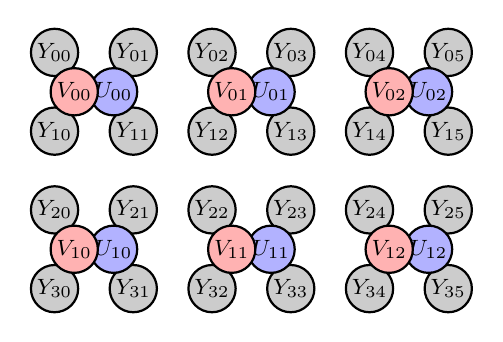
\begin{tikzpicture}
\foreach \i in {0,1,...,3} {
  \foreach \j in {0,1,...,5} {
    \draw[thick,fill=gray!40] (\j,-\i)node{\footnotesize $Y_{\i\j}$} circle(.3cm);
  }
}
\foreach \j in {0,1,2} {
  \foreach \i in {0,1} {
    \draw[thick,fill=blue!30] (2*\j+.75,-2*\i-.5)node{\footnotesize $U_{\i\j}$} circle(.3cm);
    \draw[thick,fill=red!30] (2*\j+.25,-2*\i-.5)node{\footnotesize $V_{\i\j}$} circle(.3cm);
  }
}
%\draw (2.5,-3.5)node{\footnotesize campionatura 4:2:0 di un'immagine 6x4 pixel};
\end{tikzpicture}}

\newcommand{\block}[5]{\draw[thin,fill=#1!#5] (#2,#3) rectangle +(.9,-.9) node[midway]{\footnotesize #4};}

\newcommand{\YUVplanesLuma}{
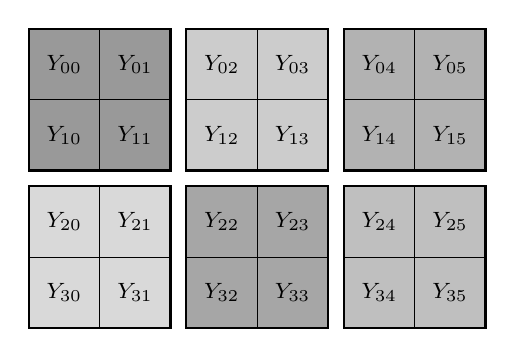
\begin{tikzpicture}

\block{gray}{0}{0}{$Y_{00}$}{80}\block{gray}{.9}{0}{$Y_{01}$}{80}
\block{gray}{0}{-.9}{$Y_{10}$}{80}\block{gray}{.9}{-.9}{$Y_{11}$}{80}
\draw[thick] (0,0)rectangle+(1.8,-1.8);

\block{gray}{2}{0}{$Y_{02}$}{40}\block{gray}{2.9}{0}{$Y_{03}$}{40}
\block{gray}{2}{-.9}{$Y_{12}$}{40}\block{gray}{2.9}{-.9}{$Y_{13}$}{40}
\draw[thick] (2,0)rectangle+(1.8,-1.8);

\block{gray}{4}{0}{$Y_{04}$}{60}\block{gray}{4.9}{0}{$Y_{05}$}{60}
\block{gray}{4}{-.9}{$Y_{14}$}{60}\block{gray}{4.9}{-.9}{$Y_{15}$}{60}
\draw[thick] (4,0)rectangle+(1.8,-1.8);

\block{gray}{0}{-2}{$Y_{20}$}{30}\block{gray}{.9}{-2}{$Y_{21}$}{30}
\block{gray}{0}{-2.9}{$Y_{30}$}{30}\block{gray}{.9}{-2.9}{$Y_{31}$}{30}
\draw[thick] (0,-2)rectangle+(1.8,-1.8);

\block{gray}{2}{-2}{$Y_{22}$}{70}\block{gray}{2.9}{-2}{$Y_{23}$}{70}
\block{gray}{2}{-2.9}{$Y_{32}$}{70}\block{gray}{2.9}{-2.9}{$Y_{33}$}{70}
\draw[thick] (2,-2)rectangle+(1.8,-1.8);

\block{gray}{4}{-2}{$Y_{24}$}{50}\block{gray}{4.9}{-2}{$Y_{25}$}{50}
\block{gray}{4}{-2.9}{$Y_{34}$}{50}\block{gray}{4.9}{-2.9}{$Y_{35}$}{50}
\draw[thick] (4,-2)rectangle+(1.8,-1.8);

%\draw (2.5, -4.5)node{\footnotesize piano per i campioni luminanza};
\end{tikzpicture}}

\newcommand{\YUVpanesCroma}{
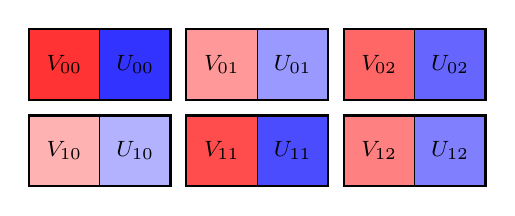
\begin{tikzpicture}
\block{red}{7}{-1}{$V_{00}$}{80}\block{blue}{7.9}{-1}{$U_{00}$}{80}
\draw[thick] (7,-1)rectangle+(1.8,-.9);

\block{red}{9}{-1}{$V_{01}$}{40}\block{blue}{9.9}{-1}{$U_{01}$}{40}
\draw[thick] (9,-1)rectangle+(1.8,-.9);

\block{red}{11}{-1}{$V_{02}$}{60}\block{blue}{11.9}{-1}{$U_{02}$}{60}
\draw[thick] (11,-1)rectangle+(1.8,-.9);

\block{red}{7}{-2.1}{$V_{10}$}{30}\block{blue}{7.9}{-2.1}{$U_{10}$}{30}
\draw[thick] (7,-2.1)rectangle+(1.8,-.9);

\block{red}{9}{-2.1}{$V_{11}$}{70}\block{blue}{9.9}{-2.1}{$U_{11}$}{70}
\draw[thick] (9,-2.1)rectangle+(1.8,-.9);

\block{red}{11}{-2.1}{$V_{12}$}{50}\block{blue}{11.9}{-2.1}{$U_{12}$}{50}
\draw[thick] (11,-2.1)rectangle+(1.8,-.9);

%\draw(9.5, -4.5)node{\footnotesize piano per i campioni crominanza};
\end{tikzpicture}}

\newcommand{\blockA}[5]{\draw[thin,fill=#1!#5] (#2,#3) rectangle +(.5,-.5) node[midway]{\tiny #4};}
\newcommand{\YUVbytestream}{
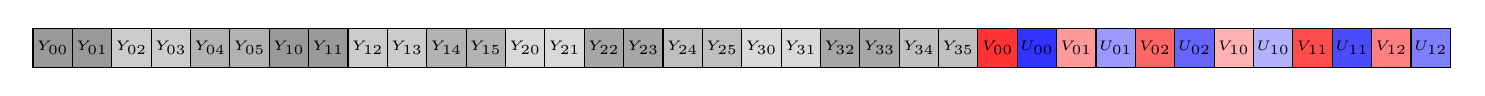
\begin{tikzpicture}
\blockA{gray}{0.0}{0}{$Y_{00}$}{80}\blockA{gray}{0.5}{0}{$Y_{01}$}{80}
\blockA{gray}{1.0}{0}{$Y_{02}$}{40}\blockA{gray}{1.5}{0}{$Y_{03}$}{40}
\blockA{gray}{2.0}{0}{$Y_{04}$}{60}\blockA{gray}{2.5}{0}{$Y_{05}$}{60}
\blockA{gray}{3.0}{0}{$Y_{10}$}{80}\blockA{gray}{3.5}{0}{$Y_{11}$}{80}
\blockA{gray}{4.0}{0}{$Y_{12}$}{40}\blockA{gray}{4.5}{0}{$Y_{13}$}{40}
\blockA{gray}{5.0}{0}{$Y_{14}$}{60}\blockA{gray}{5.5}{0}{$Y_{15}$}{60}
\blockA{gray}{6.0}{0}{$Y_{20}$}{30}\blockA{gray}{6.5}{0}{$Y_{21}$}{30}
\blockA{gray}{7.0}{0}{$Y_{22}$}{70}\blockA{gray}{7.5}{0}{$Y_{23}$}{70}
\blockA{gray}{8.0}{0}{$Y_{24}$}{50}\blockA{gray}{8.5}{0}{$Y_{25}$}{50}
\blockA{gray}{9.0}{0}{$Y_{30}$}{30}\blockA{gray}{9.5}{0}{$Y_{31}$}{30}
\blockA{gray}{10.0}{0}{$Y_{32}$}{70}\blockA{gray}{10.5}{0}{$Y_{33}$}{70}
\blockA{gray}{11.0}{0}{$Y_{34}$}{50}\blockA{gray}{11.5}{0}{$Y_{35}$}{50}

\blockA{red}{12.0}{0}{$V_{00}$}{80}\blockA{blue}{12.5}{0}{$U_{00}$}{80}
\blockA{red}{13.0}{0}{$V_{01}$}{40}\blockA{blue}{13.5}{0}{$U_{01}$}{40}
\blockA{red}{14.0}{0}{$V_{02}$}{60}\blockA{blue}{14.5}{0}{$U_{02}$}{60}
\blockA{red}{15.0}{0}{$V_{10}$}{30}\blockA{blue}{15.5}{0}{$U_{10}$}{30}
\blockA{red}{16.0}{0}{$V_{11}$}{70}\blockA{blue}{16.5}{0}{$U_{11}$}{70}
\blockA{red}{17.0}{0}{$V_{12}$}{50}\blockA{blue}{17.5}{0}{$U_{12}$}{50}

\end{tikzpicture}}

\newcommand{\securityProtocol}{
\begin{tikzpicture}
\draw (0,0) node[above]{\footnotesize RICHIEDENTE ({$\color{red}key$})} -- (0, -5);
\draw (6,0) node[above]{\footnotesize DELEGATO} -- (6, -5);
\draw (12,0) node[above]{\footnotesize SERVER ({$\color{red}key$})} -- (12, -5);

\draw[->,>=latex'] (0,-1) -- (6,-1)node[above,midway]{\footnotesize \texttt{HelloMessage}({$\color{blue}ID$})};
\draw[<-,>=latex'] (0,-2) -- (6,-2)node[above,midway]{\footnotesize \texttt{KeyRequest}($lng,lat$)};
\draw[->,>=latex'] (0,-3) -- (6,-3)node[above,midway]{\footnotesize \texttt{KeyResponse}($AES_{\color{red}key}(lng,lat)$)};
\draw[->,>=latex'] (6,-4) -- (12,-4)node[above,midway]{\footnotesize \texttt{[POST] /api/phones/{$\color{blue}ID$}/position/delegated}};
\draw[->,>=latex'] (6,-4) -- (12,-4)node[anchor=north,midway]{\footnotesize\{$AES_{\color{red}key}(lng,lat), lng,lat$\}};
\draw (12,-5)node[anchor=north]{\footnotesize $AES^{-1}_{\color{red}key}(AES_{\color{red}key}(lng,lat)) =\!\!\!\!?\;\; (lng,lat)$};
\end{tikzpicture}}
